\subsection{Undervisning}
Undervisnings delen i programmet består af to 'Usercontrols' og to 'Windows'.
Af 'Usercontrols' eksistere 'StudyTeacher' som er det et medlem med undervisning eller admin status kan se.
Den anden 'Usercontrol' er 'StudyStudent' hvilket er den studenter har adgang til, hvis man hverken er student, underviser eller admin har man således ikke adgang til nogle af disse. 
'StudyStudent' er programmeringsmæssigt meget begrænset i det dens eneste funktion er at repræsentere den enkelte students information, hvilket kun er tilgængelig for student på et read-only niveau.
I 'StudyTeacher' delen kan en underviser oprette lektioner og hold, slette hold, ændre på hold samt fuldføre uddannelsesforløbet ved at angive studenter deres duelighedsbevis.

\subsubsection{Brugergrænsefladen}
\paragraph*{StudyTeacher}
\begin{figure}[htbp]
  \centering
  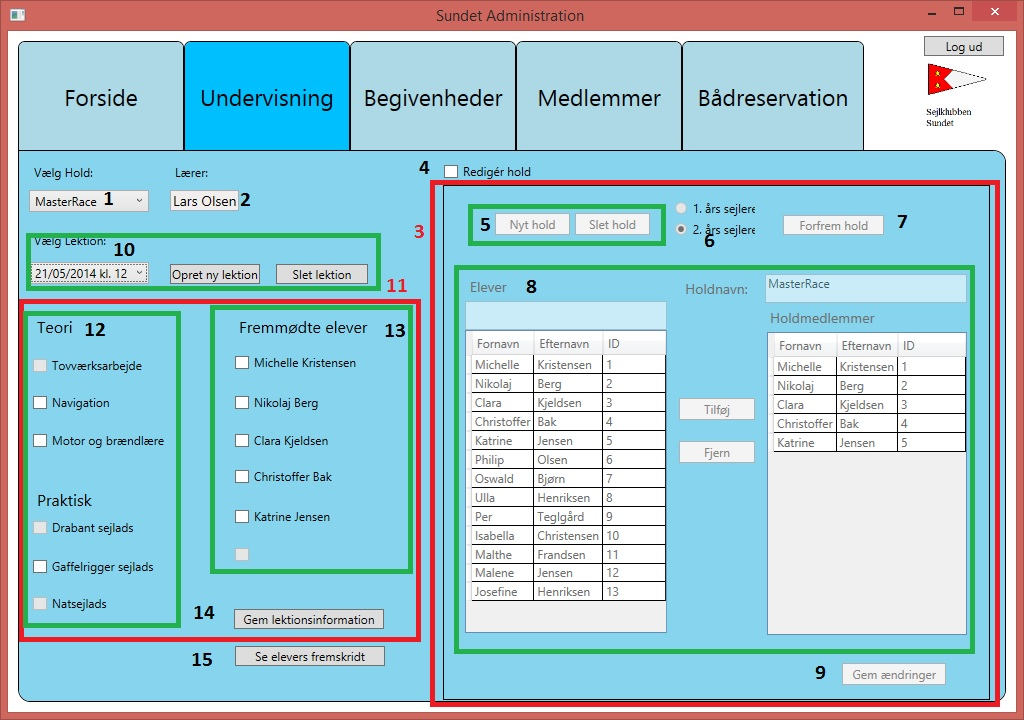
\includegraphics[width=1\textwidth]{images/UI/StudyTeacherMarked.jpg}
  \caption[UIStudyTeacher]{UI for undervisning tab som underviser og admin, markeringer bruges til forklaringer nedenfor}
  \label{fig:StudyTeacher}
\end{figure}

På \myref{fig:StudyTeacher} ses en 'Usercontrol' for 'StudyTeacher' på de markerede områder ses grupperinger af brugergrænsefladens funktioner som er sammenhængende.
\textbf{1} Referere til en 'ComboBox' som benyttes til valg af hold. 
Denne 'ComboBox' har indflydelse på det meste af undervisningsdelen, da denne information er afhængig af hvilket hold, som er valgt.
\textbf{2} Henviser til en 'CheckBox', som har kontrol over \textbf{3}, et 'Grid' indeholdende funktionalitet til brug af redigering samt kreation af hold.
\textbf{4} er tilføjning og sletning af hold, slet hold knappen sletter det hold som er valgt i \textbf{1}, mens nyt hold knappen åbner et 'nested window', 'NewTeam', i programmet hvor et nyt hold kan blive oprettet.
\textbf{5} Disse 'Radio Buttons' benyttes for at vælge om holdet er 1. års eller 2. års sejlere.
\textbf{6} Dette område benyttes til at tilføje medlemmer til et hold, at fjerne dem igen ved brug af tilføj og fjern knapperne. 
Det venstre 'DataGrid' benyttes til søgning af medlemmer, i dette grid kan findes alle 'StudentMember', mens i det højre 'DataGrid' ses de studerende som der på det valgte hold i \textbf{1}.
\textbf{7} Denne knap gemmer ændringer for holdet, dette er lavet separat for at undgå kommunikation med database ved hvert klik.
\textbf{8} Denne knap forsøger at angive et duelighedsbevis til de medlemmer på det valgte hold i \textbf{1} som opfylder alle undervisningskrav.
\textbf{9} Referer til et grid med lektionsinformation, hvis der ikke er valgt en lektion i \textbf{13} er dette 'Grid' ikke muligt at benytte.
\textbf{10} Denne række af 'CheckBoxe' bruges til at krydse af hvad der er blevet undervist i på den valgte lektion, \textbf{11} benyttes ligeledes til at afkrydse hvilke elever var til stede.
\textbf{12} Fungerer for lektion ligesom \textbf{7} for hold og er lavet for samme formål.
\textbf{13} Er en 'ComboBox' som bruges til valg af lektion.
Den sidste funktion \textbf{14} åbner et nyt 'Window', 'NewLecture', hvor man kan oprette en ny lektion for det givne hold valgt i \textbf{1}.

\paragraph{StudyStudent}

\begin{figure}[htbp]
  \centering
  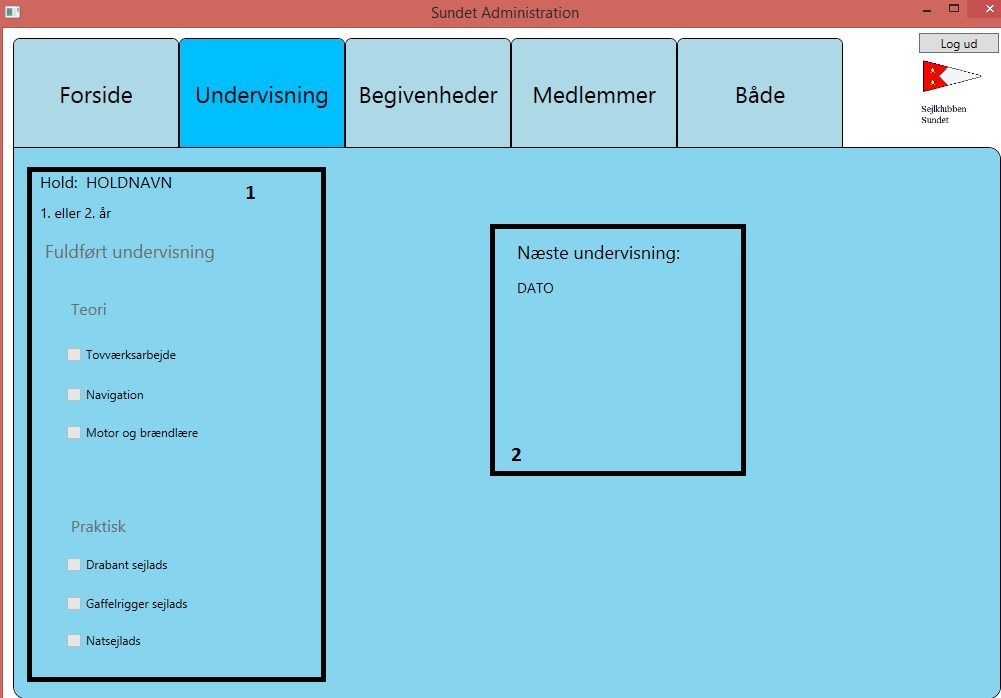
\includegraphics[width=1\textwidth]{images/UI/StudyStudentMarked.jpg}
  \caption[UIStudyStudent]{UI for undervisning tab som student, markeringer bruges til forklaringer nedenfor}
  \label{fig:StudyStudent}
\end{figure}

På \myref{fig:StudyStudent} ses en 'Usercontrol' for 'StudyStudent'. \textbf{1} Indeholder information omkring personens undervisning, 'CheckBox'ene' indikere undervisningsområder for den student som er logget ind, mens texten ovenfor viser hvilket hold personen er på. \textbf{2} Viser den næste lektionstidspunkt for det hold studenten er tilknyttet.

\paragraph{NewLecture og NewTeam}

\begin{figure}[htbp]
\centering
\begin{minipage}{.5\textwidth}
  \centering
  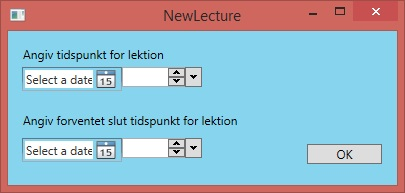
\includegraphics[width=0.8\textwidth]{images/UI/NewLecture.jpg}
  \caption[UINewLecture]{UI for NewLecture window}
  \label{fig:NewLecture}
\end{minipage}%
\begin{minipage}{.5\textwidth}
  \centering
  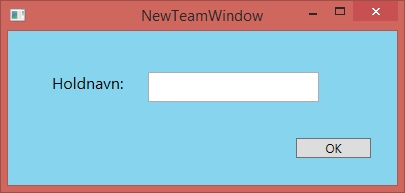
\includegraphics[width=0.8\textwidth]{images/UI/NewTeam.jpg}
  \caption[UINewTeam]{UI for NewTeam window}
  \label{fig:NewTeam}
\end{minipage}%
\end{figure}

På \myref{fig:NewLecture} ses et 'Window' for 'NewLecture'. 
I 'NewLecture' vælges der to datoer ud i fremtiden, disse bruges til at oprette en lektion, dette sker når der trykkes 'OK'. 
På \myref{fig:NewTeam} ses 'NewTeam', her skrives et holdnavn i tekstboksen, og således kan et hold oprettes.

\subsubsection{Code-Behind}
\paragraph{StudyTeacher}
\paragraph{StudyStudent}
'StudyStudent' har absolut ingen interaktion med brugeren, al koden i denne Usercontrol ligger i 'InitializeComponent' sektionen, hvilket består af at sætte den visuelle information som er tilgængelig for brugeren, ses på \myref{fig:StudyStudent}, til brugerens korrekte værdi. Det meste af dette foregår gennem en simpel assignment, enkelte værdier indeholder lidt mere logig som kan ses på \label{StudyStudentCode}. Kodeeksemplet viser 2 labels der sættes til at indeholde den korrekte string. første label, linje 5 - 7, angiver om holdet eleven er på er af 1. eller 2. år ved brug af en 'conditional operator'. den næste label, 8 - 11, benytter flere 'lambda expressions' for at finde den næste lektion i forhold til computerens tidsindstilling, denne DateTime bliver implicit casted til en string grundet linje 8'es '"" + ...' konvention.
\begin{lstlisting}[caption={Kode for at initialisere 'StudyStudent'.}\label{StudyStudentCode}]
public StudyStudent()
        {
            InitializeComponent();
			...
            level.Text = ((StudentMember) GlobalInformation.CurrentUser)
            .AssociatedTeam.Level == Team.ClassLevel.First
            ? "1. års sejlerhold" : "2. års sejlerhold";
            nextSessionDate.Text = "" +
                (((StudentMember) GlobalInformation.CurrentUser)
                 .AssociatedTeam.Lectures.OrderBy(lect => lect.DateOfLecture))
                 .FirstOrDefault(lect => lect.DateOfLecture > DateTime.Now);
        }
\end{lstlisting}

\paragraph{NewLecture}
'NewLecture' er for brugeren simpel at benytte, der er dog mere funktionalitet i dette vindue end der bliver vist for brugeren.

\begin{lstlisting}[caption={Kode for 'OK' knap i 'NewLecture' 'Window'.}\label{NewLectOk}]
private void CompleteLectureCreate_Click(object sender, RoutedEventArgs e)
        {
            var lecture = new Lecture
            {
                DateOfLecture = DateTimePickerPlannedLectureTime.Value
            };
            DalLocator.LectureDal.Create(lecture);
            var Departure = DateTimePickerPlannedLectureTime.Value;
            var Arrival = DateTimePickerPlannedLectureTimeEnd.Value;
            var book = new CreateBoatBookingWindow(Departure, Arrival, _currentTeam);
        }
\end{lstlisting}
I \myref{NewLectOk} ses koden for at trykke på OK knappen i 'NewLecture' vinduet. DateTimePicker bliver aflæst og informationen brugt til at oprette en 'Lecture', yderligere bliver informationen også gemt i henholdsvis 'Departure' og 'Arrival'. Disse bliver således videresendt i en constructer for booking af både, 'CreateBoatBookingWindow()'. Dette er OK knappens indirekte funktionalitet, funktionaliteten af dette kan ses på \myref{IndirekteBook}.

\begin{lstlisting}[caption={Dette kode bliver indirekte udført når der trykkes på 'OK' knappen, og opretter en bådreservation for lektionen.}\label{IndirekteBook}]
public CreateBoatBookingWindow(DateTime departure, DateTime arrival, Team currentTeam) 
	   : this(-1)
        {
            List<Boat> boats = new List<Boat>();
            boats = DalLocator.BoatDal.GetAll().ToList();
            Boat Anya = new Boat
            {
                Type = (currentTeam.Level == Team.ClassLevel.Second) ? BoatType.Gaffelrigger 
                : BoatType.Drabant
            };

            Boat currentBoat = boats.FirstOrDefault(
                x => x.Type == Anya.Type);

            BoatComboBox.SelectedIndex = boats.FindIndex(b => b == currentBoat);
            CrewList.Add(GlobalInformation.CurrentUser);
            CaptainComboBox.SelectedIndex = 0;
            foreach (var member in currentTeam.TeamMembers)
            {
                CrewList.Add(member);
            }
            DateTimeStart.Value = departure;
            DateTimeEnd.Value = arrival;
            PurposeTextBox.Text = "Undervisning af:" + currentTeam.Name;
            SaveButton_Click(new object(), new RoutedEventArgs());
        }
\end{lstlisting}
Denne constructer nedarver fra 'CreateBoatBookingWindow()' constructeren som kun tager en paramter, index, hertil benyttes ': this(-1)', ses på linje 2, for at sætte ComboBox'en, der styrer valg af booking, kan ses på <indsæt reference til BoatBooking>\fxnote{look at <>}, til null.
Alt efter om sejler holdet er et 1. eller 2. års sejlerhold, skal der bookes henholdsvis en drabant eller en gaffelrigger, dette håndteres på linje 6 - 15. Der laves en lokal båd, Anya, hvis 'BoatType' bliver sat gennem en 'conditional operator'.
Herefter benyttes et 'lambda expression' til at finde den første båd af den korrekte type i databasen og 'BoatComboBox', som styrer valg af båd, bliver sat til denne.
Efterfølgende bliver den admin eller underviser der opretter lektionen sat som kaptajn, det medsendte hold tilføjes 'CrewList', Departure og Arrival sættes også til de medsendte værdier, Formål bliver sat til undervisning og til sidst kaldes det event som fuldfører bookningen.